\part{Primary Classes}

{\LARGE Class List }

%{\large

	\begin{itemize}
		
		\item Server \\
			? \textit{represents the entire server�s driver code}
					
			\begin{itemize}
				\item GameLogic \\
					? \textit{Maintain the game state}
					? \textit{Keeps track of whose turn it is, etc.}
	
					\begin{itemize}
						\item Dice \\
							? \textit{Provides a means of determining spaces to move (simulates Die or spinner)}\\
							? \textit{Only contains a method that returns a random number between 1-6}
						
						\item GameBoard \\
									? \textit{Maintains and manages logical model of game board}
										
							\begin{itemize}
								\item Rooms \\
									? \textit{An array of (rooms, passage, board-location) tuples}
									? \textit{An array of non-spaces tuples}
									
								\item Pieces \\
									? \textit{An array of (player, location) tuples}
									
							\end{itemize}
							
						\item Cards \\
							? \textit{An array to hold the weapon, room, character cards}
						
					\end{itemize}
	
				\item Users \\
					? \textit{Keep track of who is connected, and what their state 
						is (connected/playing, connected/non-playing, etc) } 
					
					\begin{itemize}
						\item ServerListener \\
							? \textit{Handles initial connection requests from the clients} \\
							? \textit{All communications after initial are handled by ClientListener in Player class}
					
						\item Player \\
							? \textit{Maintains and manages server-side instance(s) of a connected player}
							? \textit{Threaded}
							
							\begin{itemize}
								\item ClientSocket \\
									? \textit{Handles socket communications with each player}
									
							\end{itemize}
					\end{itemize}
			\end{itemize}
		
		\item Client \\
			? \textit{Represents the entire client-side driver code}
			
			\begin{itemize}
				\item BoardModel \\
					? \textit{Maintains and manages model of game board to render in Gui}
					
				\item ClientSocket \\
					? \textit{maintains socket connection with server}
					
				\item GUI \\
					? \textit{Maintains and manages Graphical display}
					
					\begin{itemize}
						\item \{vast collection of support classes\} \\
							? \textit{The buttons, labels, containers, eventHandlers, etc.}
							
					\end{itemize}
			\end{itemize}
			
	\end{itemize}

%} %close \large directive from file-top

\newpage 

{\LARGE Class Diagram}

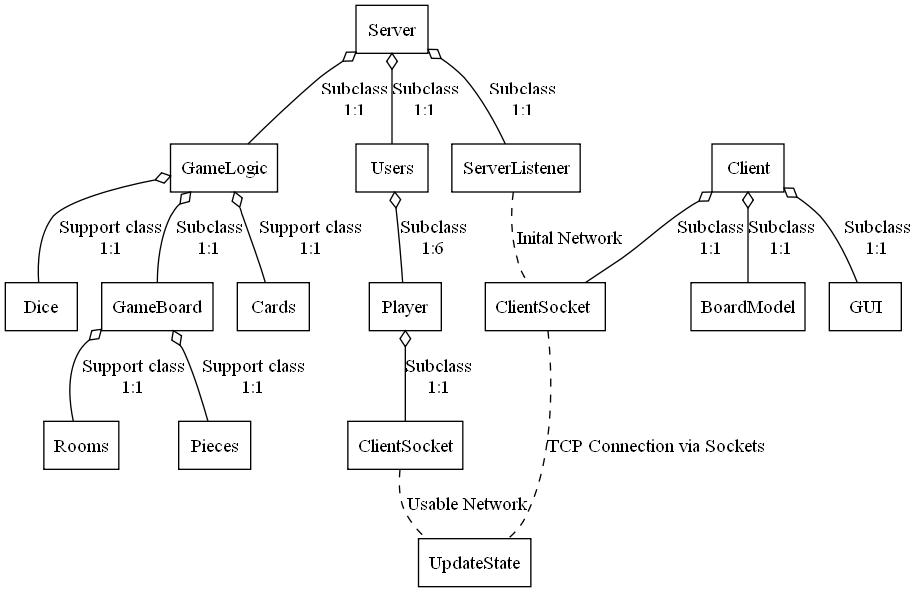
\includegraphics[scale=0.6,angle=90]{../DesignDocumentation/03_ClassList/primaryClasses2.jpg}

% \newpage
% 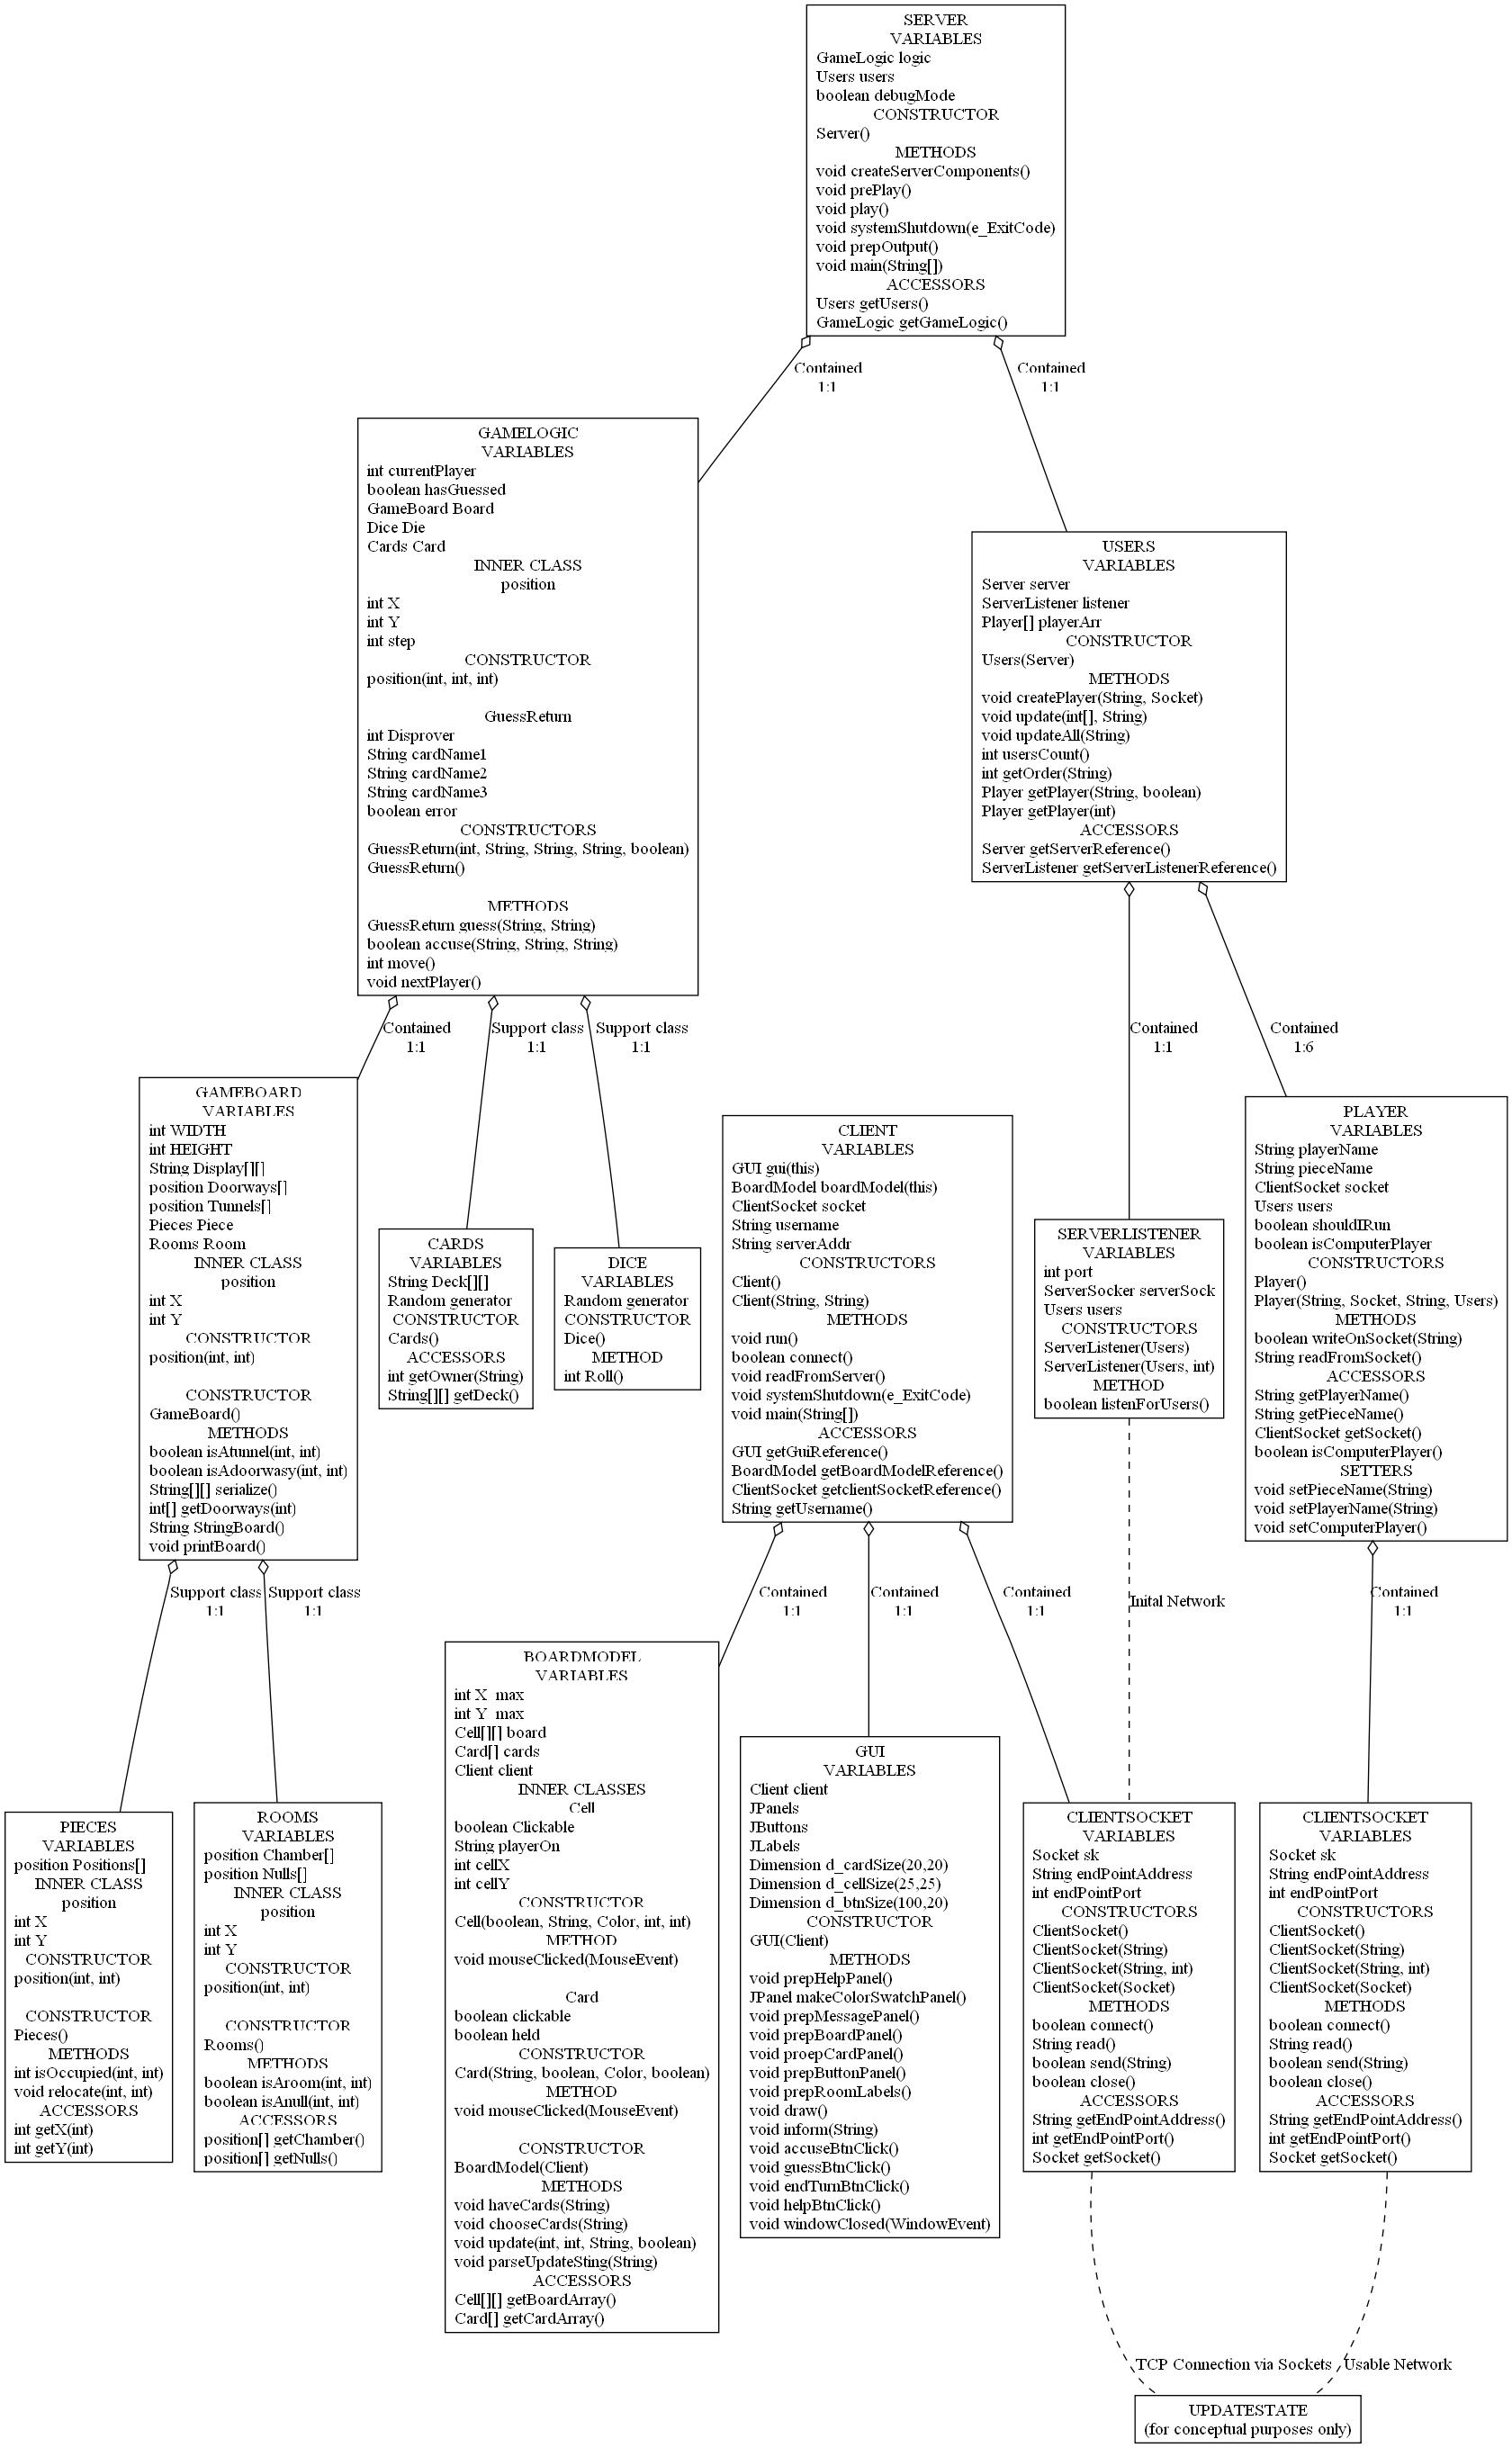
\includegraphics[scale=0.6,angle=90]{../DesignDocumentation/03_ClassList/classDiagram_FINAL_FULL.jpg}